\section{The (Sub)Universe of Finite Types}
\label{sec:ufin}

In the previous section, we have picked a particular encoding of finite types: as sequences of elements in some
canonical order.

This is not a ``free'' presentation. Some properties of the encoding might pollute our semantics. We want to make that
any theorems / properties of the semantics we prove apply to the source language (under various interpretations).

This motivates us to use a different semantic representation: a univalent universe of finite types which contains the
finite types and nothing but the finite types and is defined such as alternative representations of finite types are
identified. This guarantees that we can get a proper, sound and complete, semantics for our language.


\begin{center}
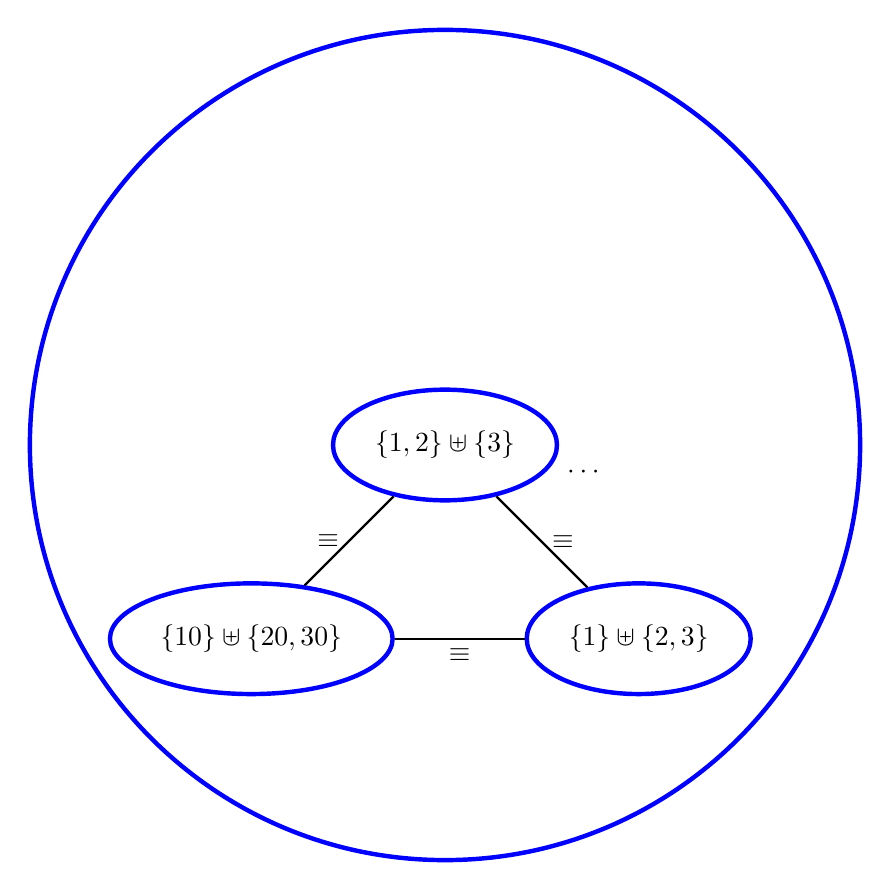
\begin{tikzpicture}[scale=1,every node/.style={scale=1}]
\usetikzlibrary{arrows}
\usetikzlibrary{shapes}
\node[ultra thick, draw=blue, ellipse, minimum width=300pt, minimum height=300pt, align=center] {};
\node[ultra thick, draw=blue, ellipse, minimum width=70pt, minimum height=40pt, align=center] (a) {$\{ 1 , 2 \} \uplus \{ 3 \}$};
\node[ultra thick, draw=blue, ellipse, minimum width=70pt, minimum height=40pt, align=center] (b) at ([shift=({70pt,-70pt})]a) {$\{ 1 \} \uplus \{ 2, 3 \}$};
\node[ultra thick, draw=blue, ellipse, minimum width=70pt, minimum height=40pt, align=center] (c) at
([shift=({-70pt,-70pt})]a) {$\{ 10 \} \uplus \{ 20, 30 \}$};
\node (d) at ([shift=({50pt,-10pt})]a) {$\cdots$};
\draw[thick,-] (a) to node[draw=none,right] {$\equiv$} (b);
\draw[thick,-] (b) to node[draw=none,below] {$\equiv$} (c);
\draw[thick,-] (a) to node[draw=none,left] {$\equiv$} (c);
\end{tikzpicture}
\end{center}

Given an operational model of how a type A reduces to a type B
Given a denotational model of which types A and B are equivalent
Want soundness and completeness results
Guarantee that the two notions of equality are themselves “equivalent”
Generalized “identity of indiscernibles”

Previous semantics adequate for reasoning about evaluation and for checking the equivalence of two circuits.

Want NBE, want rewriting system of program equivalence, what else? So we need to move to proof-relevant higher-category
groupoid semantics instead of set-theoretic.

Now the question is, what does it mean for a compiler?

My opinion is that it is still the same, what rewrites to apply depends
on the choices made by the compiler writer, but we can think about that.

%%%
\subsection{Univalent Subuniverses}
\label{sec:univalent}

In order to define the semantics, we seek a mathematical structure satisfying the following properties: (i) it contains structures corresponding to all the finite types and nothing but the finite types, and (ii) it is robust enough to ensure that equivalent encodings of finite types are identified. \note{Is this the correct informal explanation of Ufin?}

 In this section, we introduce some basic concepts and notation that we use in Homotopy Type Theory. Then, we define
univalent subuniverses and discuss some specific examples.

\subsection{The Type Theory}~\label{subsec:type-theory}

We work in Homotopy Type Theory, in particular, intensional Martin-L\"{o}f Type Theory, with a univalent universe, and
Higher Inductive Types (HITs) for propositional truncations and set quotients. We recall a few basic facts to
familiarise the reader with the notation we use. For more details about basics of HoTT, we refer the reader to the HoTT
book~\cite{univalentfoundationsprogramHomotopyTypeTheory2013}.

\note{It is important that we work in HoTT using it as a metatheory, we care about proof relevance, constructivity, and
  working with higher-dimensional algebraic structures, such as groupoids. Our results are also formalised using general
  tools and principles from HoTT, and computer checked using a proof assistant, using Agda and the HoTT-Agda library.}

\subsubsection{Identity Types}

\vc{I'm explaining everything starting from the categorical language. We do care more about the groupoid structure of
  types, and how to encode groupoids using types, since that's what we use in~\cref{sec:finite}.}

In HoTT, the intensional identity type is the type of paths between two terms of the same type. Given two terms $x:A$
and $y:A$, we write $x \id_{A} y$, or simply $x \id y$, for the equality type between them. In book HoTT, the identity
type is generated by reflexivity $\refl_{x}$, and the eliminator for the identity type is given by path induction or the
$J$-rule. The identity type equips each type with the structure of an infinity groupoid, or a homotopy type.

\todo{Say why it is a groupoid by listing some groupoid laws.}

Functions between types are functors between groupoids. Given a function $f : A \to B$, the functorial action is given
by

\[
  \term{ap}_{f} : \dfun{x,y:A}{x \id_{A} y \to f(x) \id_{B} f(y)}
\]

Type families are functions from a type to the universe, that is, an indexed family of groupoids. The $\term{transport}$
operation gives the functorial action of paths in the indexing type, which is defined by path induction. If
$P : A \to \UU$ is a type family, then for a path $x \id_{A} y$, we have

\[
  \transport{P} : \dfun{x,y:A}{x \id_{A} y \to P(x) \to P(y)}
\]

\todo{Why is the topological viewpoint important, or saying fibrations? Explain the intuition using classifying spaces,
  maybe draw some diagrams.}

From the topological viewpoint, a type family can also be seen as a fibration. For a type family $P : A \to \UU$ and a
point $x : A$, $P(x)$ gives the fiber over $a$. For a path $p : x \id_{A} y$, $\transport{P}{p}$ gives the path lifting
operation. The total space is given by $\dsum{x:A}{P(x)}$ and the first projection ${\pi_1 : \dsum{x:A}{P(x)} \to A}$ to
the base space is the fibration. The lifting operation lifts paths in the base space to paths in the total space. If
$p : x \id_{A} y$ is a path in the base space, and $u : P(x)$, we have

\[
  \term{lift}(u,p) : (x , u) \id_{\dsum{x:A}{P(x)}} (y , \tr{p}{u})
\]

where $\tr{p}{u}$ is shorthand for $\transport{P,p}(u)$.

Further, using the groupoid structure of $A$, we can show that transport lifts paths to equivalences, we define

\[
  \tptEqv{P} : \dfun{x,y:A}{x \id_{A} y \to P(x) \eqv P(y)}
\]

\todo{Explain motivation.}

\begin{definition}[Univalent Fibration]
  $P$ is a univalent type family (or simply a univalent fibration) if $\tptEqv{P}$ is an equivalence.
\end{definition}

\subsubsection{Univalence}

Voevodsky's \emph{univalence} principle characterises paths in the universe. It says that equivalent types are equal, or
the following function is an equivalence.

\[
  \ua : A \id_{\UU} B \to A \eqv B
\]

\todo{Revise.}

Alternatively, one can say that the identity type family $\term{id} : \UU \to \UU$ is univalent.

\subsubsection{Higher Inductive Types}

\todo{Explain homotopy types, $\hProp$, $\hSet$, etc.}

\vc{These are placeholder definitions, need informal explanations and references to the book.}

\begin{definition}[Propositional Truncation]
  Given a type $A$, the propositional truncation $\Trunc[-1]{A}$, or simply $\Trunc{A}$, is a higher inductive type
  generated by the following constructors,
  \begin{itemize}
    \item an inclusion function $\trunc{\blank} : A \to \Trunc{A}$,
    \item for each $x, y : \Trunc{A}$, a path $\term{trunc}(x,y) : x \id_{\Trunc{A}} y$,
  \end{itemize}
  such that, given any type $B$ with
  \begin{itemize}
    \item a function $g : A \to B$,
    \item for each $x, y : B$, a path $\term{trunc*}(x,y) : x \id_{B} y$,
  \end{itemize}
  there is a unique function $f : \Trunc{A} \to B$ such that,
  \begin{itemize}
    \item $f(\trunc{a}) \equiv g(a)$
    \item for each $x, y : \Trunc{A}$, $\ap{f}{\term{trunc}(x,y)} \id_{B} \term{trunc*}(f(x),f(y))$.
  \end{itemize}
\end{definition}

\begin{definition}[Set Quotient]
  Given a type $A$ which is an $\hSet$, and a relation $R : A \to A \to \hProp$, the set-quotient $\quot{A}{R}$ is the
  higher inductive type generated by
  \begin{itemize}
    \item an inclusion function $q : A \to \quot{A}{R}$,
    \item for each $x, y : A$ such that $R(x,y)$, a path $q(x) \id_{\quot{A}{R}} q(y)$,
    \item a set truncation, for each $x, y : \quot{A}{R}$ and $r, s : x \id_{\quot{A}{R}} y$, we have $r \id s$,
  \end{itemize}
  with \review{an appropriate induction principle.}
\end{definition}

We recall that quotients in HoTT are \emph{effective}, that is, if $R$ is an equivalence relation, we have
$R(x,y) \eqv (q(x) \id_{\quot{A}{R}} q(y))$.

\subsection{Univalent Subuniverses}

\todo{Explain motivation. Starting from a univalent universe which classifies all types, we want to define a subuniverse
  which classifies only certain types, for example, types that satisfy some property that we want.}

\begin{definition}[Universe]
  A universe \`{a} la Tarski is given by the following pieces of data,
  \begin{itemize}
    \item a code $U : \UU$,
    \item a decoding function $\El : U \to \UU$.
  \end{itemize}
  If $\El$ is a univalent fibration, $U$ is a univalent universe.
\end{definition}

\begin{definition}[Subuniverse]
  A subtype is a type family $P : \UU \to \UU$ whose fibers are prop-valued, that is, $\forall x, \isProp{P(x)}$. A
  subuniverse generated by a subtype has $U \defeq \dsum{X:\UU}{P(X)}$ and $\El \defeq \fst$.
\end{definition}

\begin{proposition}[Univalent Subuniverse]
  Subuniverses generated by subtypes are univalent.
\end{proposition}

\begin{proof}
  Suppose $(U, \El) \defeq (\dsum{X:\UU}{P(X)}, \fst)$ is a subuniverse generated by a subtype $P : \UU \to \UU$. For
  any $X, Y : \UU$ such that $\phi : P(X)$ and $\psi : P(Y)$, we want to show that
  $\tptEqv{\fst} : (X,\phi) \id (Y,\psi) \to X \eqv Y$ is an equivalence. We construct
  $X \eqv Y \to (X,\phi) \id (Y,\psi)$ by $\ua$ and using the fact that $P(\blank)$ is a proposition. That it is an
  inverse follows by calculation using the appropriate computation rules.
\end{proof}

\begin{example}[$\BAut$]
  The type of self-equivalences on a type $T$ is defined as $\Aut[T] \defeq T \eqv T$, which is an $\infty$-group. The
  subuniverse of types that are merely equal to $T$ is given by $\BAut[T] \defeq \Sub{T}$. This turns out to be the
  classifying space of $\Aut[T]$, as justified by~\cref{lem:loop-deloop}. We write $T_{o} \defeq (T, \trunc{\refl_{T}})$
  for the image of the inclusion of $T$.
\end{example}

\begin{example}
  The univalent subuniverse of types merely equal to $\Bool$ is given by $\BAut[\Bool]$. This can be used to give the
  denotational semantics of a 2-bit reversible language~\cite{caretteReversibleProgramsUnivalent2018}.
\end{example}

\begin{definition}[$\Fin$]
  The type family $\Fin : \Nat \to \UU$ is the type of finite sets indexed by cardinality. It is defined equivalently in
  two different ways,
  \begin{gather*}
    \begin{aligned}
      \Fin[n] & \defeq \dsum{k:\Nat}{k < n}
    \end{aligned}
    \begin{aligned}
      & \Fin[0] \defeq \bot \\
      & \Fin[\suc[n]] \defeq \top \sqcup \Fin[n]
    \end{aligned}
  \end{gather*}
  Note that $\Fin[n]$ is a $\hSet$, and we use the definitions interchangeably.
\end{definition}

\begin{example}
  For any $n : \Nat$, we define the univalent subuniverse of types merely equal to $\Fin[n]$ as $\BAut[\Fin[n]]$. This
  is the universe of finite sets with cardinality equal to $n$. We write $F_{n} \defeq (\Fin[n], \trunc{\refl})$ for the
  image of the inclusion of $\Fin[n]$.
\end{example}

\begin{definition}[$\isFin$]
  We say that a type is finite if it is merely equal to $\Fin[n]$ for some $n$.
  \[
    \isFin[X] \defeq \dsum{n:\Nat}{\SubP{X}{\Fin[n]}}
  \]
  Note that the natural number $n$ need not be truncated, as justified below.
\end{definition}

\begin{proposition}
  For any type $X$, $\isFin[X]$ is a proposition.
\end{proposition}

\begin{proof}
  Suppose we have $(n,\phi) : \isFin[X]$ and $(m,\psi) : \isFin[X]$, we need to show that $(n,\phi) \id (m,\psi)$. It is
  enough to show that $n \id m$. Since $\Nat$ is a set, this is a proposition, so we can use the induction principle of
  propositional truncation to eliminate to $n \id m$, applying it on $\phi$ and $\psi$ respectively. This gives us the
  equalities $X \id \Fin[n]$ and $X \id \Fin[m]$, which gives us $\Fin[n] \id \Fin[m]$, from which $n \id m$ follows by
  applying the first projection.
\end{proof}

\begin{example}
  The univalent subuniverse of \emph{all finite types} is given by
  \[
    \UFin \defeq \dsum{X:\UU}{\isFin[X]}.
  \]
  We write $F_{n} \defeq (\Fin[n], n, \trunc{\refl})$, for the image of the inclusion of $\Fin[n]$. We use this as the
  denotational semantics to interpret our reversible programming language $\PiPlusLang$.
\end{example}

\review{We characterise the path space of univalent subuniverses.}

\begin{proposition}
  If $T$ is an $n$-type, $\BAut[T]$ is an $(n+1)$-type.
\end{proposition}

\begin{proof}
  We need to show that the equality type of $\BAut[T]$ is an $n$-type. Assume $X, Y : \BAut[T]$. Since $\BAut[T]$ is a
  univalent subuniverse, we have $(X \id Y) \eqv (\fst(X) \eqv \fst(Y))$. Note that being an $n$-type is a proposition.
  Since $T$ is an $n$-type, and $\fst(X)$ and $\fst(Y)$ are merely equal to $T$, they're also $n$-types. It follows that
  $\fst(X) \eqv \fst(Y)$ is an $n$-type, and hence $X \id Y$ is an $n$-type.
\end{proof}

\begin{proposition}
  For any $T : \UU$, $\BAut[T]$ is 0-connected.
\end{proposition}

\begin{corollary}
  $\UFin$ is a pointed, connected, 1-type, that is, a 1-groupoid, or has h-level 3.
\end{corollary}

\begin{lemma}~\label{lem:loop-deloop}
  \[
    \loopspace[\BAut[T],T_{0}] \eqv \Aut[T]
  \]
\end{lemma}

\begin{proof}
  Since $\BAut[T]$ is a univalent universe, it follows that
  \[
    (T_{0} \id_{\BAut[T]} T_{0}) \eqv (\fst(T_{0}) \eqv \fst(T_{0})) \equiv (T \eqv T) \equiv \Aut[T].
  \]
\end{proof}

\begin{corollary}
  For every $n:\Nat$,
  \[
    \loopspace[\UFin[n],F_{n}] \eqv \Aut[\Fin[n]]
  \]
\end{corollary}

\subsection{Rig structure}~\label{subsec:rig}

\todo{rig}

We describe the symmetric monoidal structure of the groupoid $\UFin$.

First, we observe a few equivalences.

\begin{proposition}
  For any $n, m : \Nat$,
  \begin{align*}
    \Fin[0]                & \eqv \bot \\
    \Fin[n] \sqcup \Fin[m] & \eqv \Fin[n + m] \\
  \end{align*}
  and for any types $X, Y, Z$,
  \begin{align*}
    \bot \sqcup X          & \eqv X \\
    X \sqcup \bot          & \eqv X \\
    (X \sqcup Y) \sqcup Z  & \eqv X \sqcup (Y \sqcup Z) \\
    X \sqcup Y             & \eqv Y \sqcup Y \\
  \end{align*}
\end{proposition}

We lift these equivalences to $\UFin$ giving it the (additive) symmetric monoidal structure $(I, \oplus)$, with natural
isomorphisms $\lambda_{X}$, $\rho_{X}$, $\alpha_{X,Y,Z}$, and the symmetry isomorphism $\mathcal{B}_{X,Y}$. Note that
types in $\UFin$ are $\hSet$s since they're merely equivalent to $\Fin[n]$ for some $n : \Nat$.

\begin{definition}
  \begin{align*}
    I           & \defeq F_{0}    \\
    X \oplus Y & \defeq X \sqcup Y \\
    \lambda_{X} & : I \oplus X \eqv X \\
    \rho_{X} & : X \oplus I \eqv X \\
    \alpha_{X,Y,Z} & : (X \oplus Y) \oplus Z \eqv X \oplus (Y \oplus Z) \\
    \mathcal{B}_{X,Y} & : X \oplus Y \eqv Y \oplus X
  \end{align*}
\end{definition}

These isomorphisms satisfy the Mac Lane coherence conditions for symmetric monoidal categories, that is, the triangle,
pentagon, and hexagon identities, and the syllepsis of the braiding, upto 2-paths in $\UFin$.

\begin{proposition}
  % https://q.uiver.app/?q=WzAsNCxbMCwwLCIoWCBcXG9wbHVzIEkpIFxcb3BsdXMgWSJdLFsyLDAsIlggXFxvcGx1cyAoSSBcXG9wbHVzIFkpIl0sWzEsMSwiWCBcXG9wbHVzIFkiXSxbMCwxXSxbMCwxLCJcXGFscGhhX3tYLEksWX0iXSxbMCwyLCJcXHJob197WH0gXFxvcGx1cyAxX3tZfSIsMl0sWzEsMiwiMV97WH0gXFxvcGx1cyBcXGxhbWJkYV97WX0iXSxbNSw2LCJcXGlkIiwwLHsic2hvcnRlbiI6eyJzb3VyY2UiOjIwLCJ0YXJnZXQiOjIwfSwic3R5bGUiOnsiYm9keSI6eyJuYW1lIjoibm9uZSJ9LCJoZWFkIjp7Im5hbWUiOiJub25lIn19fV1d
  \[\begin{tikzcd}
      {(X \oplus I) \oplus Y} && {X \oplus (I \oplus Y)} \\
      {} & {X \oplus Y}
      \arrow["{\alpha_{X,I,Y}}", from=1-1, to=1-3]
      \arrow[""{name=0, anchor=center, inner sep=0}, "{\rho_{X} \oplus 1_{Y}}"', from=1-1, to=2-2]
      \arrow[""{name=1, anchor=center, inner sep=0}, "{1_{X} \oplus \lambda_{Y}}", from=1-3, to=2-2]
      \arrow["\id", Rightarrow, draw=none, from=0, to=1]
    \end{tikzcd}\]
  % https://q.uiver.app/?q=WzAsNSxbMCwxLCIoKFcgXFxvcGx1cyBYKSBcXG9wbHVzIFkpIFxcb3BsdXMgWiJdLFsxLDAsIihXIFxcb3BsdXMgWCkgXFxvcGx1cyAoWSBcXG9wbHVzIFopIl0sWzIsMSwiVyBcXG9wbHVzIChYIFxcb3BsdXMgKFkgXFxvcGx1cyBaKSkiXSxbMiwzLCJXIFxcb3BsdXMgKChYIFxcb3BsdXMgWSkgXFxvcGx1cyBaKSJdLFswLDMsIihXIFxcb3BsdXMgKFggXFxvcGx1cyBZKSkgXFxvcGx1cyBaIl0sWzAsMSwiXFxhbHBoYV97VyBcXG9wbHVzIFgsIFksIFp9Il0sWzEsMiwiXFxhbHBoYV97VyxYLFkgXFxvcGx1cyBafSJdLFszLDIsIjFfe1d9IFxcb3BsdXMgXFxhbHBoYV97WCxZLFp9IiwyXSxbMCw0LCJcXGFscGhhX3tXLFgsWX0gXFxvcGx1cyAxX3tafSIsMl0sWzQsMywiXFxhbHBoYV97VyxYIFxcb3BsdXMgWSxafSIsMl0sWzAsMiwiXFxpZCIsMSx7Im9mZnNldCI6NSwic3R5bGUiOnsiYm9keSI6eyJuYW1lIjoibm9uZSJ9LCJoZWFkIjp7Im5hbWUiOiJub25lIn19fV1d
  \[\begin{tikzcd}
      & {(W \oplus X) \oplus (Y \oplus Z)} \\
      {((W \oplus X) \oplus Y) \oplus Z} && {W \oplus (X \oplus (Y \oplus Z))} \\
      \\
      {(W \oplus (X \oplus Y)) \oplus Z} && {W \oplus ((X \oplus Y) \oplus Z)}
      \arrow["{\alpha_{W \oplus X, Y, Z}}", from=2-1, to=1-2]
      \arrow["{\alpha_{W,X,Y \oplus Z}}", from=1-2, to=2-3]
      \arrow["{1_{W} \oplus \alpha_{X,Y,Z}}"', from=4-3, to=2-3]
      \arrow["{\alpha_{W,X,Y} \oplus 1_{Z}}"', from=2-1, to=4-1]
      \arrow["{\alpha_{W,X \oplus Y,Z}}"', from=4-1, to=4-3]
      \arrow["\id"{description}, shift right=5, draw=none, from=2-1, to=2-3]
    \end{tikzcd}\]
  % https://q.uiver.app/?q=WzAsNixbMSwwLCJYIFxcb3BsdXMgKFkgXFxvcGx1cyBaKSJdLFswLDEsIihYIFxcb3BsdXMgWSkgXFxvcGx1cyBaIl0sWzAsMiwiKFkgXFxvcGx1cyBYKSBcXG9wbHVzIFoiXSxbMSwzLCJZIFxcb3BsdXMgKFggXFxvcGx1cyBaKSJdLFsyLDIsIlkgXFxvcGx1cyAoWiBcXG9wbHVzIFgpIl0sWzIsMSwiKFkgXFxvcGx1cyBaKSBcXG9wbHVzIFgiXSxbMSwwLCJcXGFscGhhX3tYLFksWn0iXSxbMSwyLCJcXG1hdGhjYWx7Qn1fe1gsWX0gXFxvcGx1cyAxX3tafSIsMl0sWzIsMywiXFxhbHBoYV97WSxYLFp9IiwyXSxbMyw0LCIxX3tZfSBcXG9wbHVzIFxcbWF0aGNhbHtCfV97WCxafSIsMl0sWzUsNCwiXFxhbHBoYV97WSxaLFh9Il0sWzAsNSwiXFxtYXRoY2Fse0J9X3tYLFkgXFxvcGx1cyBafSJdLFs3LDEwLCJcXGlkIiwwLHsic2hvcnRlbiI6eyJzb3VyY2UiOjIwLCJ0YXJnZXQiOjIwfSwic3R5bGUiOnsiYm9keSI6eyJuYW1lIjoibm9uZSJ9LCJoZWFkIjp7Im5hbWUiOiJub25lIn19fV1d
  \[\begin{tikzcd}
      & {X \oplus (Y \oplus Z)} \\
      {(X \oplus Y) \oplus Z} && {(Y \oplus Z) \oplus X} \\
      {(Y \oplus X) \oplus Z} && {Y \oplus (Z \oplus X)} \\
      & {Y \oplus (X \oplus Z)}
      \arrow["{\alpha_{X,Y,Z}}", from=2-1, to=1-2]
      \arrow[""{name=0, anchor=center, inner sep=0}, "{\mathcal{B}_{X,Y} \oplus 1_{Z}}"', from=2-1, to=3-1]
      \arrow["{\alpha_{Y,X,Z}}"', from=3-1, to=4-2]
      \arrow["{1_{Y} \oplus \mathcal{B}_{X,Z}}"', from=4-2, to=3-3]
      \arrow[""{name=1, anchor=center, inner sep=0}, "{\alpha_{Y,Z,X}}", from=2-3, to=3-3]
      \arrow["{\mathcal{B}_{X,Y \oplus Z}}", from=1-2, to=2-3]
      \arrow["\id", Rightarrow, draw=none, from=0, to=1]
    \end{tikzcd}\]
  % https://q.uiver.app/?q=WzAsMyxbMCwwLCJYIFxcb3BsdXMgWSJdLFsyLDAsIlggXFxvcGx1cyBZIl0sWzEsMSwiWSBcXG9wbHVzIFgiXSxbMCwxLCIxX3tYIFxcb3BsdXMgWX0iLDAseyJsZXZlbCI6Miwic3R5bGUiOnsiaGVhZCI6eyJuYW1lIjoibm9uZSJ9fX1dLFswLDIsIlxcbWF0aGNhbHtCfV97WCxZfSIsMl0sWzIsMSwiXFxtYXRoY2Fse0J9X3tZLFh9IiwyXSxbNCw1LCJcXGlkIiwwLHsic2hvcnRlbiI6eyJzb3VyY2UiOjIwLCJ0YXJnZXQiOjIwfSwic3R5bGUiOnsiYm9keSI6eyJuYW1lIjoibm9uZSJ9LCJoZWFkIjp7Im5hbWUiOiJub25lIn19fV1d
  \[\begin{tikzcd}
      {X \oplus Y} && {X \oplus Y} \\
      & {Y \oplus X}
      \arrow["{1_{X \oplus Y}}", Rightarrow, no head, from=1-1, to=1-3]
      \arrow[""{name=0, anchor=center, inner sep=0}, "{\mathcal{B}_{X,Y}}"', from=1-1, to=2-2]
      \arrow[""{name=1, anchor=center, inner sep=0}, "{\mathcal{B}_{Y,X}}"', from=2-2, to=1-3]
      \arrow["\id", Rightarrow, draw=none, from=0, to=1]
    \end{tikzcd}\]
\end{proposition}

%%% Local Variables:
%%% mode: latex
%%% TeX-master: "main"
%%% fill-column: 120
%%% End:
